\documentclass[thesis]{cluu}

\usepackage[style=cluu]{biblatex}
\usepackage{tabularx}
\usepackage[acronym]{glossaries}
\usepackage{tikz}
\usetikzlibrary{arrows.meta,positioning,shapes.geometric,fit}
\usepackage{cleveref}
\usepackage{graphicx}
\graphicspath{ {./images/} }
\usepackage{adjustbox}
\usepackage{hyperref}
%\usepackage[nameref]

\makeglossaries

\newacronym{ai}{AI}{Artificial Intelligence}
\newacronym{ml}{ML}{Machine Learning}
\newacronym{nlp}{NLP}{Natural Language Processing}
\newacronym{call}{CALL}{Computer-Assisted Language Learning}
\newacronym{icall}{icall}{Intelligent CALL}
\newacronym{capt}{CAPT}{Computer-Assisted Pronunciation Training}
\newacronym{json}{JSON}{JavaScript Object Notation}
\newacronym{llm}{LLM}{Large Language Model}
\newacronym{nlg}{NLG}{Natural Language Generation}
\newacronym{md}{MD}{Mispronunciation Detection}
\newacronym{mdd}{MDD}{Mispronunciation Detection and Diagnosis}
\newacronym{ctc}{CTC}{Connectionist Temporal Classification}
\newacronym{cnn}{CNN}{Convolutional Neural Network}
\newacronym{sota}{SotA}{State-of-the-Art}
\newacronym{fleurs}{FLEURS}{Few-shot Learning Evaluation of Universal Representations of Speech}
\newacronym{l2}{L2}{second language}
\newacronym{l1}{L1}{first language}
\newacronym{sla}{SLA}{second-language acquisition}
\newacronym{nn}{NN}{neural network}
\newacronym{tts}{TTS}{Text-to-Speech}
\newacronym{asr}{ASR}{automatic speech recognition}
\newacronym{ipa}{IPA}{the International Phonetic Alphabet}
\newacronym{g2p}{G2P}{Grapheme-to-Phoneme}
\newacronym{wals}{WALS}{the World Atlas of Linguistic Structure}
\newacronym{mfa}{MFA}{Montreal Forced Aligner}
\newacronym{mt}{MT}{Machine Translation}
\newacronym{tl}{TL}{Transfer Learning}
\newacronym{mooc}{MOOC}{massive open online course}
\newacronym{e2e}{E2E}{end-to-end}
\newacronym{gop}{GOP}{goodness of pronunciation}
\newacronym{gmm}{GMM}{Gaussian Mixture Model}
\newacronym{hmm}{HMM}{hidden Markov model}

% Define tikz styles to reuse in figures
\usepackage[edges]{forest}
\usetikzlibrary{arrows.meta} % for Latex arrowheads

\forestset{
  box/.style={
    draw, rounded corners=2mm, thick,
    minimum height=9mm, align=center
  },
  internal/.style={box, fill=blue!10},
  posleaf/.style={box, fill=green!15},
  negleaf/.style={box, fill=red!15},
  edgelabel/.style={midway, sloped, above},
}

% Define a new counter for paragraphs (delete when paper is done)
\newcounter{paranum}
% Command to increment and display the paragraph number for initial planning
\newcommand{\numberedparagraph}{\par\refstepcounter{paranum}\textbf{[\theparanum] }}

\newcommand{\todo}[1]{\textcolor{red}{#1}}

% use Doulos SIL for IPA transcriptions
\newfontfamily\ipafont{Doulos SIL}[Scale=MatchLowercase]
\newcommand{\ipa}[1]{{\ipafont #1}}

%ThesisProject is auto updated by zotero
\addbibresource{ThesisProject.bib}

\begin{document}
\title{My thesis}
\author{Peter Cady}
% \date{...}
\supervisors{Johan Sjons, Uppsala University\\
  Jim O' Regan, KTH Royal Institution of Technology}
% Use \supervisor (without s at end) if you have only one

\maketitle

\begin{abstract}
    \numberedparagraph{summarize the motivation}
    \numberedparagraph{problem overview}
    \numberedparagraph{experiment}
    \numberedparagraph{main findings and contributions.}
\end{abstract}

\tableofcontents

\addchap{Preface}
% with \addchap instead of \chapter it isn't numbered.
\addchap{Acknowledgements}
Thank my partner
Thank Johan
I would especially like to thank Jim O' Regan for all his thought-provoking insights, encouragement, and advice, which were crucial for me getting my bearings in a project which pushed me to grow well beyond my limits. The process was deeply meaningful to me. Thank you.
Thank Greg
I would like to thank my Irish professor Gregory Darwin for his commitment and engagement in promoting Irish literature and the Irish language 
Thank examiner

\printglossary[type=\acronymtype]

\printglossary

\chapter{Introduction}
\numberedparagraph{Lead work here. Outline modern context of minority languages in nlp. Introduce Irish context in this framework.}
\todo{revisit introduction, try to lead with an impactful framing of the motivation of the work.}
Language competency is crucial for securing opportunities in the workplace as well as for accessing services and exercising rights in society at large. As our surroundings become ever more digitally interconnected, these interactions are increasingly mediated by language technologies, for both good and ill. Such technologies are often identified as promising tools to promote language use and language learning, but are also implicated in the coalescence of online interaction around a few dominant languages such as English, complicating the glowing promises often offered by their proponents. Low-resource language communities struggle to keep pace with the most recent technological advancements given the relative scarcity of resources they are faced with, necessitating approaches tailored to these limitations if the true promise of cutting-edge language technologies is to be realized for these groups most in need. The momentum of the pre-training/fine-tuning paradigm within \gls{asr} and \gls{ml} more generally in recent years offers a glimmer of hope to those working toward making accessible tools for such communities, enabling the use of more plentiful data to support tools for languages facing varying levels of resource scarcity.

\numberedparagraph{Reiterate need for a solution, lead into research questions.} 
Promoting speech technologies for language learning could be of particular benefit for languages such as Irish which struggle to propagate native models of speech effectively to motivated learners outside of traditionally Irish-speaking areas. Through \gls{capt} applications built with careful use of the aforementioned, we might find the scaleable, resource con

\numberedparagraph{RQ's} 
To this end, in this work we explore two potential avenues to overcoming the data limitations faced by Irish and other languages like it: one, by using the data we \textit{do} have by harnessing readily available monolingual data in a model ensemble; and the other, by imitating the data we \textit{wish} we had with \gls{tts}-generated learner approximations to train a model with. These approaches are formulated concretely as:
\begin{enumerate}
  \item To what extent can a resource-conscious ensemble of monolingual ASR models (Irish and English) approach the performance of a high-resource upper-bound model trained on fully annotated mispronunciation data (L2-ARCTIC)?
  \item To what extend can a model trained on TTS-generated synthetic mispronunciation data approach the performance of a high-resource upper-bound trained on fully annotated learner mispronunciation data (L2-ARCTIC)?
\end{enumerate}

\numberedparagraph{Outline key goals of thesis, give a "road map" for what's to come.}
In this thesis we explore the feasibility of two primary methods of overcoming the scarcity of phonetically annotated \gls{l2} Irish learner data for \gls{md} applications. One approaches the problem with ensembles of monolingual \gls{asr} models for which data scarcity less acute, and another using a schema of data generation by leveraging established \gls{tts} systems to approximate learner speech: a potential low-cost alternative to large-scale phonetic annotation. By exploring these approaches, we aim to illuminate possible ways forward for low-resource language communities interested in developing automated technologies for language learning and pronunciation training.


\chapter{Background}
\numberedparagraph{Short overview of background section}

In the following section we will outline the context motivating our current work with relation to \gls{nlp} and \gls{asr} research for minority languages. We begin by summarizing the state of minority languages in current research, highlighting some promising trends as well as some thusfar recalcitrant problems hindering more equal access to the benefits of our time's rapid advances in language technology. We then proceed to outline the more general research space of the current work: \gls{call} and \gls{capt} before digging into the core task of \gls{capt} systems: \gls{md} and \gls{mdd}. We conclude with a technical overview of modern \gls{asr} systems used for such tasks, leaving the specific efforts of researchers to overcome data limitation inherent to low-resource languages in the next section, \todo{get chapter and section references working}%\nameref{chap:Related Work}.

\section{Irish \& The Predicament of Minority Languages in Natural Language Processing (NLP)}

\numberedparagraph{introduce need for general-use systems.}

Developing language technologies that can scale beyond the language they are designed for is no new goal for \gls{nlp} research. The value of such a property is apparent: transferring an existing system seamlessly to another language could potentially save significant resources for language communities without the ability to fund such system development themselves. Actually achieving this goal in practice, however, is no simple endeavor, typically requiring some level of linguistic awareness which is all-to-often lamentably absent \parencite[see][inter alia]{benderAchievingEvaluatingLanguageIndependence2011,joshiStateFateLinguistic2021,hedderichSurveyRecentApproaches2021}. For example, success in applying supposedly language independent word-based n-gram approaches to languages rests on its level of inflectional morphology: the lower the better. Higher morphological complexity together with variations in word order raise data sparsity problems which n-gram approaches rooted in English struggle to handle \parencite{benderAchievingEvaluatingLanguageIndependence2011}. This should come as no surprise, given the relatively fixed word order and low levels of inflectional morphology present in English, but it illustrates a need for caution: systems developed for a given language may make implicit assumptions about language structure which do not generalize well.\todo{add concrete example to illustrate? maybe exemplify more directly from above reference} Linguistic typology can provide important clues as to what features are shared between the original development language and possible languages of extension for a system. Information of this kind has, for many of the worlds languages, already been gathered by linguists. Perhaps the most renowned database of typological information is \gls{wals} \parencite{matthewdryerWorldAtlasLanguage2024}, a free, online resource currently boasting 152 chapters with detailed descriptions of 192 linguistic features spanning over 2,600 of the world's languages. How a language is communicated through script is also a point of complication for \gls{nlp} research, with \textcite{manoharWhatLostNormalization2024} implicating standard normalization praxis when comparing ASR models as artificially inflating scores of languages using Indic scripts. Correctly segmenting continuous-script languages like Chinese is another area of ongoing research with clear implications for downstream performance. \todo{cut this. text work is not directly relevant to my project, and it doesn't illuminate any particular point.}. By explicitly mobilizing linguistic knowledge already painstakingly gathered by linguistic typologists, we can identify where languages agree, where they differ, and hopefully identify implicit, ungeneralizable assumptions underpinning our approaches earlier in the design stage.

\numberedparagraph{language disparity in lang tech.} 
Despite the claims of language-agnostic systems often touted by proponents of emerging \gls{ai} technologies, these systems have often fallen well short of such promise \parencite{benderAchievingEvaluatingLanguageIndependence2011}\todo{add some examples of where to read further + inter alia}. The overwhelming majority of the world's languages have no footprint in emerging language technologies \parencite{joshiStateFateLinguistic2021}. In the past, building \gls{nn}-based language technologies has demanded immense quantities of labeled data: a high bar of entry to the language communities of those languages with limited if any access to such resources, and an ongoing issue which continues to stimulate a body of research dedicated to overcoming such issues(see \textcite{magueresseLowresourceLanguagesReview2020} for an overview). For languages where data availability is no obstacle, research and development can proceed unfettered by the prohibitive cost of curating datasets from scratch. As our daily lives grow increasingly integrated with the digital realm, language communities without the same support are obliged to switch to more digitally dominant languages (often English) to gain access to these new resources, narrowing the opportunities to engage with resources and services through the medium of their community language \parencite{nichasaideCanWeDefuse2019}. A particularly sobering taxonomy illustrating the states of languages facing such disparities is formulated by \textcite{joshiStateFateLinguistic2021} and reproduced in \cref{tab:data_availability} on page \pageref{tab:data_availability}, which outlines the states and challenges faced by languages in resource terms in the digital space, and how dominant a small group of languages are within it. Of particular note for the privileged few that find themselves at the top of the heap is their typological similarity, being drawn as they are from a few dominant language families (and even dominant branches within these larger families). This state of affairs constitutes a sort of typological echo-chamber for the cutting edge of \gls{nlp} developments, a point which we will return to shortly.

\begin{table}[h]
    \centering
    \begin{tabularx}{\textwidth}{|X|p{2cm}|p{1.75cm}|}
        \hline
        \textbf{Class Descriptions} & \textbf{Example Languages} & \textbf{\% of total languages}\\ \hline
        \textbf{0} The Left-Behinds: Virtually ignored in language technology. Exceptionally limited resources available, even with respect to unlabeled data. & Dahalo, Bora & 88.17\%\\ \hline
        \textbf{1} The Scraping-Bys: Some unlabeled data. With organized promotion and data collection, there is hope for improvement in coming years. & Fijian, Navajo & 8.93\%\\ \hline
        \textbf{2} The Hopefuls: Limited labeled data. Support communities help these languages survive, and there is promise for \gls{nlp} tools in the near term. & Zulu, \textbf{Irish} & 0.76\%\\ \hline
        \textbf{3} The Rising Stars: Strong web presence and thriving cultural community online. Lacking in labeled data. Good potential for \gls{nlp} tool development for these languages. & Indonesian, Hebrew & 1.13\%\\ \hline
        \textbf{4} The Underdogs: Much unlabeled data, and less but still significant labeled data. Dedicated investment from NLP communities. & Russian, Dutch & 0.72\%\\ \hline
        \textbf{5} The Winners: Dominant online presence with massive investment and resources. & English, German & 0.28\%\\ \hline
    \end{tabularx}
    \caption{Data availability \& status taxonomy of languages adapted from work by \textcite{joshiStateFateLinguistic2021}.}
    \label{tab:data_availability}
\end{table}
\numberedparagraph{set the Irish case in this context, outline challenges currently undertaken by developers}

Despite some advantages not afforded other minority languages, Irish still finds itself struggling to maintain a footing in the the digital realm, placed by \textcite{joshiStateFateLinguistic2021} in class 2 of the taxonomy outlined in \cref{tab:data_availability}. It enjoys ongoing investment by the Irish state, nominal status of Irish as the first national language of the Republic of Ireland, and research dedicated to its promotion (e.g. through the ABAIR initiative dedicated to developing speech technologies for Irish, see \parencite{chasaideABAIRInitiativeBringing2017}). At the same time, it is a typological outlier in several respects: it is a verb-initial language with relatively complex inflectional morphology, and a distinct (though still Latin-based) orthography. Features like these put Irish at odds with many languages in the high-resource echo-chamber, complicating the ability to leverage cutting-edge models to linguistic features with no representation in a model's training data. Furthermore, though we have treated Irish as a single entity thus far, an important complication reveals itself in the discontiguous nature of the Irish-speaking areas, referred to as \textit{the Gaeltachtaí}. Each of the three main areas (i.e. Ulster, Connacht, and Munster \ref{fig:gaeltacht}) speak markedly distinct varieties of Irish, necessitating labeled data from each variant if these groups are to be adequately serviced by new technologies\parencite{nichasaideCanWeDefuse2019}. In the face of such limitations, today's data-hungry tools simply cannot be expected to perform to the same level on languages like Irish without the same access to resources. It should be noted that the pretraining/finetuning paradigm of recent massive multilingual models does mitigate this demand for data somewhat by leveraging unlabeled cross-lingual data, reducing the need for labeled data in the language finetuned to \parencite{hedderichSurveyRecentApproaches2021,ranathungaNeuralMachineTranslation2021,joshiStateFateLinguistic2021}, but for other languages without even minimal labeled data to their name, this is a small comfort.\todo{which survey references do I want to use?}

\begin{figure}[h]
    \caption{Area of the Gaeltachtaí (Irish-speaking areas of Ireland) colored in green}
    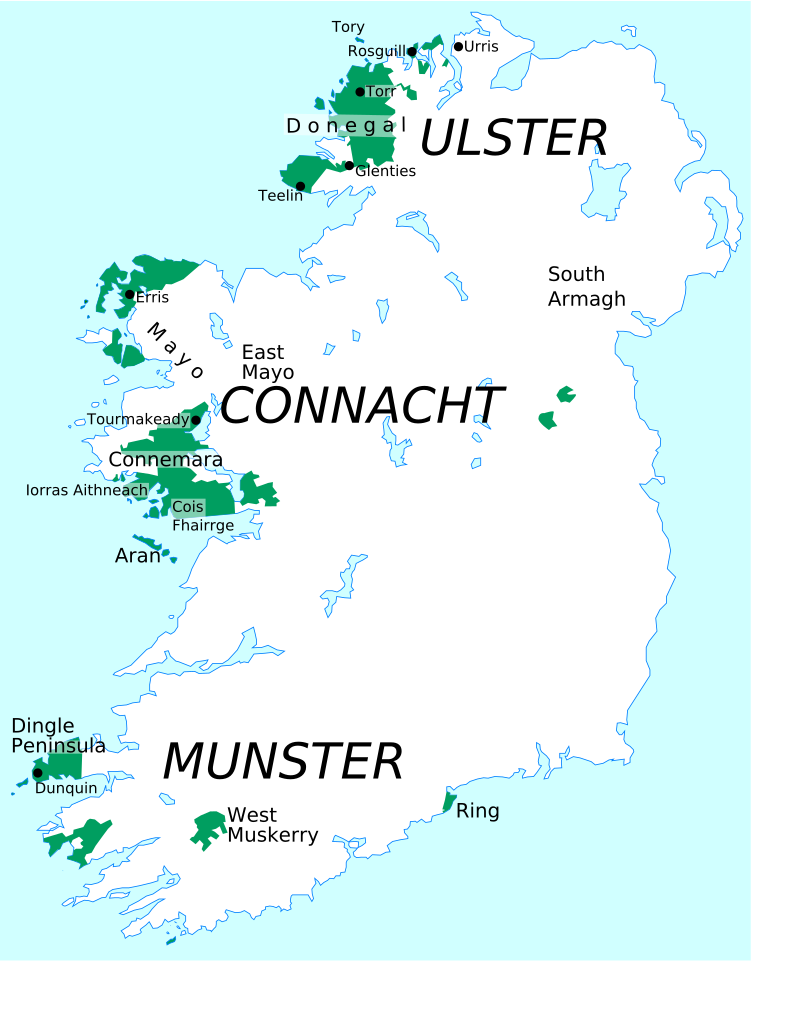
\includegraphics[width=8cm]{Gaeltachtai_le_hainmneacha2.png}
    \centering
    \label{fig:gaeltacht}
    \caption{The original uploader was Angr at English Wikipedia. - Transferred from en.wikipedia to Commons., CC BY-SA 3.0, https://commons.wikimedia.org/w/index.php?curid=3532749}
\end{figure} 

\numberedparagraph{problems to be solved for Irish speakers}
Though the hurdles facing the Irish language in the digital sphere are a relatively recent concern, the issues facing it in the real world are anything but. It is currently classified by UNESCO as being \textit{definitely endangered} \parencite{moseleyAtlasWorldsLanguages2010}, following centuries of varying rates of contraction due to encroachment by English \todo{give some more explanation of the history, handle with care}. Irish survives as a community languages in the aforementioned Gaeltacht areas, though even there it is estimated that only 24\% of inhabitants speak Irish on a daily basis \parencite{nichasaideSPEECHTECHNOLOGYDOCUMENTATION}. Despite the state of Irish as a \gls{l1}, it is comparatively strong as a \gls{l2} \todo{broinNewUrbanIrish}. A growing number of parents seek Irish-medium education for their children outside the Gaeltacht, and immersive summer courses remain popolar among adults looking to learn or reconnect with the language. This encouraging \gls{l2} engagement intersects with thorny issues of supply, however, as many of the teachers are not themselves native speakers with an accompanying native grasp of the structure and sound of the language \parencite{nichasaideSPEECHTECHNOLOGYDOCUMENTATION,nichasaideCanWeDefuse2019}. This limited native speaker model for \gls{l2} speakers is particularly problematic for teaching pronunciation, complicating the acquisition of some sound contrasts critical to disambiguating the Irish grammar. Perhaps chiefly among these, contrasts between the secondary articulation of consonants into \textit{palatalised} and \textit{velarised} variants play an instrumental role in a number of grammatical functions, such as in the formation of certain plurals and genitive marking \parencite{snesarevaPalatalizationDublinIrish2016,gabrieleEnglishInfluenceL2,broinNewUrbanIrish,stensonModernIrishComprehensive2020}. Since the Roman alphabet doesn't provide symbols for this distinction, Irish orthography marks it via adjacent letters as seen in \todo{give sub-table references} of \cref{tab:sound_contrasts}: so-called \textit{slender} vowels ('i' and 'e') flanking a consonant denote \textit{palatalisation}, while \textit{broad} vowels ('a', 'o', and 'u') mark \textit{velarisation} \parencite{stensonModernIrishComprehensive2020}. Mutation effects are another pervasive element of the Irish grammar relying on sound alterations, the most common of which are \textit{lenition} and \textit{eclipsis}. \textit{Lenition},traditionally termed \textit{séimhiú} (/\ipa{ˈʃeːvʲuː}/), is commonly marked with an 'h' following the lenited consonant as seen on \cref{tab:sound_contrasts}, and originally denoted a weakening in the manner of articulation, though the relationship between consonants and their lenited versions is less immediately apparent now for some consonants \parencite{stensonModernIrishComprehensive2020}. \textit{Eclipsis}, traditionally \textit{úru} (/\ipa{ˈʊɾˠuː}/), involves replacing the original consonant with a nasalized or voiced version, and is denoted by appending the new sound character before the consonant being eclipsed\ref{tab:sound_contrasts} \todo{add sub-table refs and double check if this description covers all the bases}. These and other structural underpinnings of the language can have far-reaching implications for intelligability if not adequately mastered by students. Indeed, a study undertaken by\textcite{broinNewUrbanIrish} reveals that realisations of phonological like those above are over 50\% on average for urban speakers, with some as high as 82\%---a stark departure from their gaeltacht counterparts which lie below 10\%. Providing wider access to better native models of pronunciation --- not to mention native models of morphology --- could do much to close this gap, making mutual intelligability more attainable between gaeltacht and urban speakers. 

\begin{table}[ht]
  \centering
  \caption{Examples use of mutation effects a. séimhiú \& b. úru as well as c. consonant velarisation \& d. palatalisation. Adapted from \textcite{nichasaideSPEECHTECHNOLOGYDOCUMENTATION}}
  \begin{tabular}{c|l|l|l|l}
     & Orthographic & \gls{ipa} & Translation \\
    \hline
    a. & bád & /\ipa{bˠaːdˠ}/ & 'boat' \\
    b. & báid & /\ipa{bˠaːdʲ}/ & 'boats' \\
    c. & do bhád & /\ipa{dˠɔ waːdˠ}/ & 'your boat'\\
    d. & ár mbád & /\ipa{ɛɾʲ mˠaːdˠ}/ & 'our boat'\\
  \end{tabular}
  \label{tab:sound_contrasts}
\end{table}

\textcite{gabrieleEnglishInfluenceL2} english influence on palatalization and velarization
\textcite{snesarevaPalatalizationDublinIrish2016} how does english influence Irish spoken by dublin bilinguals?
\textcite{broinNewUrbanIrish} differences of irish between cities and gaeltacht
\textcite{nichasaideSPEECHTECHNOLOGYDOCUMENTATION} documentation of Irish with speech tech

\textcite{magueresseLowresourceLanguagesReview2020} survey of low resource methods in \gls{nlp}
\textcite{wuTransformerBasedEndtoEnd2021} motivation for phone-based recognition for MDD instead of scoring pronunciations (like GOP)

\section{From Text to Speech: Approaches to Low-Resource Scenarios}
With the rise of \gls{nn}-based language technologies, the data-hungry nature of such tools underscores the urgency of addressing the kind of resource disparities outlined at the beginning of this chapter. Making such tools accessible to languages without the same strong data foundations as English is an active area of ongoing research, though even within popular languages such as English, non-standard domains and tasks types can constitute low-resource areas which lack suitable quantities of training data \parencite{hedderichSurveyRecentApproaches2021}. These data disparities can be categorized along several dimensions, such as those proposed by \textcite{hedderichSurveyRecentApproaches2021} for \gls{nlp} as: availability of \textit{task-specific labeled data} for the target language or domain, availability of \textit{unlabeled} language- or domain-specific data, or the availability of \textit{auxiliary} data. This latter kind of data is diverse, as it is data not directly labeled for the task at hand, but which can still be indirectly useful, from labels specific to another language/domain, to knowledge bases such as entity lists, or automated labels from \gls{mt} systems \parencite{hedderichSurveyRecentApproaches2021}.

\numberedparagraph{overview of low resource approaches}
To address the different dimensions of resource scarcity outlined above, various approaches have been developed which \textcite{hedderichSurveyRecentApproaches2021} splits broadly into those which \textit{generate additional labeled data}, and those employing \gls{tl}. Faced with limited gold-standard annotated data, researchers employ strategies of the former type to (semi-)automatically produce labeled alternatives. These strategies can be themselves broadly grouped as \textit{data augmentation}, where task-specific labeled data is used to make more labeled data, such as with Back-Translation for \gls{mt} where a target-to-source translation model is used to obtain a synthetic parallel corpus from a monolingual target corpus \parencite{ranathungaNeuralMachineTranslation2021}, and \textit{distant supervision} which produces labels for existing unlabeled data, for example in Cross-Lingual Annotation Projection where a task-specific classifier is trained for a high-resource language, then projected onto text from a low-resource language using a paralell corpus. For \gls{tl}, in contrast, instead of creating or extending task-specific training data, the focus lies on reducing the need for such data by leveraging models or learned representations from other languages/domains. This approach has been particularly successful in in recent years with the advent of models like BERT \parencite{devlinBERTPretrainingDeep2019} and Wav2Vec2 \parencite{baevskiWav2vec20Framework2020} which are \textit{pre-trained} on vast quantities of unlabeled data to then be \textit{fine-tuned} for specific downstream tasks. This pretraining/fine-tuning paradigm can be particularly advantageous for languages or domains where labeled data is limited.

\numberedparagraph{Connect these general trends to applicability in Automatic Speech Recognition}
Although these strategies are commonly employed in \gls{nlp}, analogous trends can be found in computer vision as well as speech to tackle similar limitations in data. \gls{tl} and the aforementioned pretraining/fine-tuning paradigm has made strides with self-supervised models like Wav2vec2, outperforming previous state-of-the-art \gls{asr} models with 100 times less data, starkly reducing the demand for labeled speech \parencite{baevskiWav2vec20Framework2020}. Alongside \gls{tl}, ensemble methods have also emerged as a promising tool for low-resource contexts. Here, specialist models with complementary attributes can be combined to perform better than any one of its constituents for novel tasks \parencite[inter alia]{arunkumarInvestigationEnsembleFeatures2022,dengEnsembleDeepLearning2014,gitmanConfidencebasedEnsemblesEndtoEnd2023,fiscus1997post}. Various methods of data augmentation are also prevalent to improve \gls{asr} performance for low-resource languages, including voice transformations, where noise or other alterations are introduced to recordings to extend existing data, or \gls{tts}-generated synthetic audio is used to bolster training data when authentic speech corpora are lacking \parencite{barteldsMakingMoreLittle2023,zhangL2GENNeuralPhoneme2022}.

\textcite{hedderichSurveyRecentApproaches2021} survey of low resource NLP methods
\textcite{magueresseLowresourceLanguagesReview2020} survey of low resource methods in \gls{nlp}

\section{Computer-Assisted Language Learning (CALL) \& Computer-Assisted Pronunciation Training (CAPT)}
Despite efforts to the contrary, the rise of digital technologies is often implicated in the acceleration of already precpitous rates of decline for endangered languages \todo{dig up reference to strenghten this point}. However, it is a trend that cuts both ways, as the same technologies that squeeze certain languages out of the digital realm are also making space for communities of language learners to come together towards their common goal through \gls{call} platforms and \gls{mooc}s. The increased presense of technology both in and outside the classroom brings with it broad implications for traditional pedgagogy, enabling more autonomous and flexible modes of learning for students \parencite{spolskyHandbookEducationalLinguistics2008}\todo{alter bib entry to reflect book chapter, not whole book} particularly for learners looking to autonomously improve their pronunciation
 via \gls{capt} systems. This technological shift has increased the financial viability of courses for endagered or otherwise less commonly taught languages, allowing teachers to draw from a more geographically dispersed enrollment pool and provide courses otherwise impossible to offer. Despite this potential, tension between the technology and pedagogy underpinning \gls{call} and \gls{capt} systems remains a well-documented issue \parencite{rogerson-revellComputerAssistedPronunciationTraining2021}, echoing calls for greater collaboration between pedagogical and technical experts when designing these systems.

The proliferation of \gls{call} software for self-study such as Duolingo, Babbel, and Rosetta Stone proliferate, has renewed interest in the role of immediate and personalised feeback for pronunciation training in \gls{capt} systems. Recent research indicates that language learners may need explicit and targeted feedback on their pronunciation in order to improve \parencite{bajorek2017l2}, despite the long-held understanding that error correction typically does not meaningfully influence acquisition \parencite{krashenPrinciplesPracticeSecond1984}. Perhaps as a consequence of this established view, explicit pronunciation training has been notably absent from language classrooms in recent decades, and many of these \gls{call} platforms carry on this legacy with binary right-or-wrong feedback mechanisms that do not make use of the potential for more effective, targeted feedback \parencite{bajorek2017l2}. The feedback is also frequently unexplained, making such binary judgements about pronunciation quality opaque to the student and thus more difficult to act on. This kind of individualized, explained feedback would normally carry a steep price tag for the student of an individual tutor, say, but \gls{capt} systems can potentially lower this barrier of entry considerably by automating the same kind of undivided feedback in a one-to-many form scalable to many geographically disperesed students at once. 

\section{Automatic Speech Recognition}
\numberedparagraph{general overview of ASR}
goal: transcribe speech to text \todo{not done, get good descriptors from \textcite{jurafskySpeechLanguageProcessing2025} and \textcite{yuAutomaticSpeechRecognition2015}}

\numberedparagraph{old asr models, hmm gnn}
These systems convert of an acoustic waveform into feature vectors by a signal processer, which are then combined by a decoder with a dictionary and language model or grammar network into a recognition network. Using this network, one can calculate the most likely word sequence given the waveform of the speech input \parencite{witt2000use}.
\numberedparagraph{Description of Wav2vec2 model}
\textcite{conneauUnsupervisedCrosslingualRepresentation2020} Wav2vec2 XLSR
\textcite{baevskiVqwav2vecSelfSupervisedLearning2020} (vector quantized) wav2vec2 with learned discrete representations
One popular ASR models used in extracting phonemes from raw acoustic data is currently \textit{wav2vec 2.0}, a self-supervised framework which is conceptually simpler than other leading models. After pre-training on unlabeled data, it can be fine-tuned on a much smaller set of labeled data, achieving \gls{sota} results in scenarios where labeled data is scarce \textcite{baevskiWav2vec20Framework2020}. It consists of three main components: a \gls{cnn}-based \textit{feature encoder}, a \textit{Transformer}-based network, and a \textit{quantization module}. The feature encoder takes raw audio as input and outputs latent speech representations to be used both by the Transformer network and the quantization module. The Transformer captures contextual information about the encoder output, while the quantization module divides the encoder output into discrete speech representations.\todo{adapt diagram from wav2vec2 paper and explain the components properly.}

\numberedparagraph{motivation for wav2vec2 xlsr}
The ability to pre-train on freely available unlabeled data makes Wav2Vec 2.0 a natural choice for low-resource scenarios where one cannot count on abundant labeled data to train a model from the ground up. By leveraging the benefits afforded by the pre-training/fine-tuning paradigm, we can make the most of data limited both by domain and language. \todo{not done, probably unnecessary.}
\textcite{baevskiEffectivenessSelfsupervisedPretraining2020} self supervision enabling ASR at low cost

\section{Pronunciation \& Mispronunciation Detection and Diagnosis (MDD)}
To realize the often untapped potential of \gls{capt} and lay the groundwork for actionable feedback, the \gls{asr} system must be able to identify deviations in student pronunciations from the target pronunciation and determine how it differs in ways interpretable to the student. We must first clarify what we mean by pronunciation, starting with an abstraction of the human speech apparatus as a collection of subsystems which can emit signals over parallel channels \parencite{engstrandFonetikensGrunder2004}. Although speech is a continuous signal, we can map symbols of speech sounds--phones--onto its subsegments. These discrete units---the vowels and consonants that constitute words---are \textit{segmental} features of speech. The prosody, intonation, stress, and other such elements of speech can be seen as superimposed on these segmental features, and are thus termed \textit{suprasegmental} features of speech\parencite{engstrandFonetikensGrunder2004}. Human cultures have an array of strategies for representing speech in written form, ranging from logographic writing systems like Chinese where one symbol represents one word, to different varieties of sound-based systems such as syllabic for Japanese hiragana or katakana, alphabetic like the Roman alphabet I use here, or consonantal as in Semitic scripts\parencite{jurafskySpeechLanguageProcessing2025}. For our purposes, we will narrow our investigation of \gls{md} to segmental features, representing pronunciation as strings of phones using the \gls{ipa} standard of phonetic notation. Though suprasegmental features can also play a crucial role in disambiguating meaning, investigating them is beyond the scope of this thesis.

\numberedparagraph{difference in objectives}
To 
\numberedparagraph{classical gop approaches}
Research into \gls{mdd} gained significant momentum in the 1990's to early 2000's, centering on \gls{hmm}-\gls{gmm} based \gls{asr} systems. Early approaches pronunciation scoring using these systems typically relied on log-likelihood scores and log-posterior scores \parencite{wittAutomaticErrorDetection} the latter of which eventually eclipsing the former due to its higher correlation with human assessments \todo{expand this section. explain the log-likelihood approach and posterior with equations. it will be relevant in related works when tying it to wav2vec2 outputs}. Building further on this development, \textcite{witt2000use} introduced the widely used \gls{gop} measure of pronunciation quality, which could be compared against a threshold value to determine how well the speaker's pronunciation matches the canonical model pronunciation \parencite{witt2014computer}.
\textcite{witt2000use} GOP dissertation
\textcite{sudhakaraImprovedGoodnessPronunciation2019} improved GOP
\textcite{fuFullTextDependentEnd2021} data augmentation for MDD
\textcite{kheirMispronunciationDetectionSpeechBlender} MDD with hmm gnn for arabic
\textcite{kheirAutomaticPronunciationAssessment2023} review of MDD capt systems
\textcite{kheirL1awareMultilingualMispronunciation2023} Multilingual MDD framework
\numberedparagraph{E2E ASR approaches}
More recently, \gls{e2e} \gls{nn}-based based systems like Wav2Vec2 have gained traction as promising alternatives to more traditional \gls{hmm}-\gls{gmm} approaches. Logit outputs of these models are analogous to the posterior probabilities derived from \gls{hmm}s, providing probabilities of a phoneme given the speech segment, but suffers from issues of 'peakiness' and overconfidence which complicate their interpretability as direct analogues to hmm-based posterior probabilities \parencite{parikhEvaluatingLogitBasedGOP2025} touches on confidence and peakiness\parencite{zeyerWhyDoesCTC2021} peakiness

\textcite{alrashoudiImprovingMispronunciationDetection2025} MDD for arabic with transformers
\textcite{kimAutomaticPronunciationAssessment2022} focus more on pron scoring instead of MDD
\textcite{pengStudyFineTuningWav2vec202021} Wav2vec2 for MDD (important)
\textcite{pengTextAwareEndtoendMispronunciation2022} gating strategy (ignore irrelevant parts in transcription) and constrastive loss to reduce objective gap between phoneme recognition and MDD
\textcite{shahinPhonologicalLevelMispronunciationDetection2024} phonological-level MDD (articulatory focus) True acceptance rate, false rejection tc
\textcite{stanleyImprovingL1specificPhonological2012} difference in L1 dependent models vs baseline. how to introduce non native acoustic features. (variant of min phone error training that optimizes on maximizing discriminability between confusable phonetic units in nonnative acoustic space.)
\textcite{xuExploreWav2vec202021} wav2vec2 for MDD

\parencite{barteldsMakingMoreLittle2023} survey of low-resource ASR
\parencite{besacierAutomaticSpeechRecognition2014} survey of low-resource ASR


\chapter{Related Work}
In the following section, we will dive into some strategies used to address the problem areas outlined above: recent applications of \gls{asr} in \gls{md}, as well as some of the strategies adopted to overcoming the mismatch in objectives between ordinary phoneme recognition and \gls{md} which motivate the approaches taken in the current work:
\begin{enumerate}
  \item \gls{asr} model ensembles,
  --and--
  \item \gls{tts}-generated data augmentation
\end{enumerate}

\section{ASR for MDD}


\numberedparagraph{Touch on phoneme extraction task and detail fine-tuning procedure}
\textcite{agrawalLearningWhenTrust2023} smart weighter mechanism that selects model based on input audio

\numberedparagraph{MDD scoring}

% forest package for more painless trees
\begin{figure}[t]
\centering
\begin{adjustbox}{max width=\linewidth}
\begin{forest}
for tree={
  edge={-{Latex[length=1.6mm]}},
  l sep=5mm,        % level separation (vertical)
  s sep=2mm          % sibling separation (minimum horizontal)
}
[Transcribed Phonemes, internal
  [Correct Pronunciations, internal
    [True Acceptance, posleaf]
    [False Rejection, negleaf]
  ]
  [Mispronunciations, internal
    [False Acceptance, negleaf]
    [True Rejection, internal
      [Correct Diagnosis, posleaf]
      [Diagnosis Error,  negleaf]
    ]
  ]
]
\end{forest}
\end{adjustbox}
\label{fig:eval}
\caption{Evaluation hierarchy of phoneme level \gls{md}}
\end{figure}

\section{Ensembling}
\parencite[inter alia]{barteldsMakingMoreLittle2023,zhangL2GENNeuralPhoneme2022,kheirAutomaticPronunciationAssessment2023,thaiSyntheticDataAugmentation2019}
\numberedparagraph{describe the general strategy of model ensembling}
\textcite{fiscus1997post} ROVER ensembling
\textcite{jalalvandAutomaticQualityEstimation2018} novel ROVER approach with quality ranking at segment level
\textcite{gitmanConfidencebasedEnsemblesEndtoEnd2023} confidence-based ASR ensembles with selector block

\section{TTS data augmentation}
\textcite{shenNaturalTTSSynthesis2018} TTS Tacotron (maybe find google tts paper)

\numberedparagraph{connect strategy to current work}
\textcite{punjabiLanguageModelBootstrapping2019} bootstrapping data with MT (important)
\textcite{xuIterativePseudoLabelingSpeech2020} multiple iteration of pseudo-labeling on unlabeled data to overcome data scarcity
\textcite{yangImprovingMispronunciationDetection2022} pseudo-labeling to overcome scarcity (self-superviced learning)

\textcite{khareLowResourceASR2021} transliteration as a bridge between orthographies
\textcite{korzekwaComputerassistedPronunciationTraining2022} synthesis approaches to boosting asr
\textcite{barteldsMakingMoreLittle2023} TTS + ASR boosts ASR performance
\textcite{zhangL2GENNeuralPhoneme2022} phoneme paragraphing to generate mispronounced speech (important)

\chapter{Methods \& Materials}
In the following section, we will describe the core experiments explored for the current work: one which explores model ensembling as described above as a solution to \gls{md} in the face of data scarcity; the other, which explores dataset bootstrapping with a \gls{tts} system to create the data required to train a model directly for \gls{md}. Leading this will be an overview of the model framework common to both of these experiments: Wav2vec 2.0.
\section{General Experiment Setup}
Connect the low resource dimensions and approaches to my contributions.
\numberedparagraph{teanglann, timit, tts}
\numberedparagraph{preprocessing, cleaning, etc.}
\numberedparagraph{base model description}
\section{Experiment 1: Monolingual Ensembling}
\numberedparagraph{outline first experiment with model ensemble.}
Our first experiment starts with the intuition described above using two expert systems: one Irish and one English. Confidence values associated with each models phonemic outputs are compared to each other to reach a combined phonetic output. 
\textcite{guoCalibrationModernNeural2017} predicting probability estimates. how well calibrated are our models?
\textcite{niehuesModelingConfidenceSequencetoSequence2019} similarity between training and test conditions for confidence (maybe more suitable as an extension)
\textcite{papadopoulosConfidenceEstimationMethods2001} maximum likelihood, approximate bayesian, bootstrapping. (confidence estimation assessed by mean and st dev etc.)
\textcite{weiMitigatingNeuralNetwork2022} mitigating overconfidence with logit normalization during training. some background on softmax confidence scores

\subsection{Data}
\numberedparagraph{briefly summarize data sources}
To train our monolingual systems, we procured two monolingual corpora of read speech audio with phonetic transcriptions. Our English model was trained on the TIMIT corpus \textcite{garofolo1993timit} with the Irish model trained on audio data from the online Irish Dictionary and Language Library\footnote{\url{https://www.teanglann.ie/en/}}. To evaluate effectiveness of the system for \gls{md}, a manually annotated datset was prepared from a small subsection of the Mozilla Common Voice dataset
\textcite{krishenbaumRepresentingIPAPhonetics} use is ascii is used (it's not)
\textcite{mechuraIntroductionGramadanIrish} introduction to grammar part of teanglann (maybe not relevant)

\numberedparagraph{timit}
The TIMIT corpus is a read speech corpus of American English speakers who spent their childhoods in one of eight major dialect areas of the United States. These areas are widely recognized with the exception of the Western dialect region, where boundaries are not confidently delineated, and the "army brat" group, consisting of speakers which frequently moved during their childhood due to the demands of highly mobile military service member parents, resulting in exposure to a variety of dialects. The full dataset consists of 6300 sentences from 630 speakers, so ten sentences per speaker. This 
\textcite{ardilaCommonVoiceMassivelyMultilingual2020} common voice corpus for L2 speech

\numberedparagraph{teanglann}
The Dictionary and Language Library is an online resource developed by Foras na Gaeilge\footnote{Foras na Gaeilge is a group which promotes the Irish language, supports Irish-medium education, and advises public and private sector organizations, among its other functions. \url{https://www.forasnagaeilge.ie/}} in conjunction with the New English-Irish Dictionary. Among the resources available are The Pronunciation Database, which contains recordings of individual words spoken by native speakers from three major dialects: Connacht, Ulster, and Munster. The recordings for Ulster used for our monolingual Irish model were scraped by myself, adhering to the site's robots.txt file limit of one request per two seconds. \todo{am i using MFA or the dict?} The dictionary of words to scrape was derived from an Ulster Irish \gls{g2p} file generously provided by Jim O' Regan. This was used for canonical Ulster phonetic annotation, and could be combined to form a dataset of words, recordings, and phonetic annotations in \gls{ipa} for a combined dataset duration of roughly five hours of audio.
\todo{talk to jim about where he got the g2p dict I use for pronunciation information and as a scraping dict}
\subsection{Models}
\numberedparagraph{which wav2vec2 variant I used}

\section{Experiment 2: Synthetic Mispronunciation Data}
\subsection{Data}
\textcite{zhang2022l2gen} synthetic data generation

\subsection{Models}

\section{Evaluation}
\numberedparagraph{overview, skyline, baseline}
 \textcite{graves2006connectionist} ctc loss
\numberedparagraph{data used}
\numberedparagraph{annotation details} 
To prepare the Common Voice dataset for use in phoneme-level \gls{md}, a small subset of the data was manually transcribed in \gls{ipa} to capture pronunciation deviations from standard Ulster pronunciation. The process of capturing these deviations consisted of the following steps: first, an \gls{ipa} representation of the transcription was generated from a lookup in the Ulster \gls{g2p} dictionary to map the orthographic transcriptions to their canonical \gls{ipa} representations; recordings were then manually assessed, comparing these generated \gls{ipa} representations to the audio and noting where the phonemes deviated from the canonical pronunciations and what their realization was assessed to be. This process was carried out by myself only, a notable limitation we will return to later. The annotations were carried out in Label Studio using some preliminary annotations generated by an \gls{mfa} \gls{g2p} model trained on Ulster Irish to speed up the process \todo{ask about where the g2p came from, what to reference}

\numberedparagraph{Common voice}
For evaluating the quality of the \gls{md} system, we begin with the Irish portion of the Common Voice dataset\textcite{ardilaCommonVoiceMassivelyMultilingual2020}, noted by \textcite{lonerganAutomaticSpeechRecognition} as consisting nearly entirely of \gls{l2} speakers\footnote{given its nature as a crowd-sourced dataset, it is not certain this is still the case for the Irish portion of Common Voice}. As in their work, this dataset will be used as the basis for testing the current experiment, as it fits the purpose of evaluating our system's effectiveness on \gls{l2} speech. The Common Voice corpus is a massive multilingual collection of transcribed speech designed for ASR which leverages crowd sourcing for data collection and validation to help alleviate the dirth of training data faced by most languages. 
\textcite{conneauFLEURSFewshotLearning2022} Parallel ASR dataset. move to discussion.
\textcite{deichlerMMConvMultimodalConversational2024} multimodal conversational dataset with cospeech gestures. move to discussion
\textcite{qianAutomaticSpeechRecognition2022} ASR for irish: uses Mozilla common voice
\textcite{zhangSpeechocean762OpenSourceNonnative2021} open source speech corpus speech ocean for pronunciation assessment
\textcite{zhaoL2ARCTICNonnativeEnglish2018} L2 arctic dataset
\textcite{leeMassivelyMultilingualPronunciation} wikipron (not used but illustrative as a reference)
\numberedparagraph{metrics CER, F1, etc. Detail CTC loss used in training}
CTC loss \textcite{gravesConnectionistTemporalClassification} also details some peakiness
\textcite{kurzingerCTCSegmentationLargeCorpora2020} ctc and dataset bootstrapping
\numberedparagraph{protocol, why does this enable comparison? (bridge between methods, materials, and results)}



\chapter{Results}
\numberedparagraph{detail the results as it pertains to the evaluation framework: CER}


\chapter{Discussion}
\numberedparagraph{Summarize the main findings from results and how it relates to the research questions}

\numberedparagraph{Detail possible applications to Language learning, the role of results in augmenting self-directed language learning}
\textcite{hardisonSecondlanguageSpokenWord2005} effect of multimodal input on speech identification

\numberedparagraph{Detail possible (or actual if time allows) Furhat application} 
\textcite{deichler2024mm} multimedia data

\numberedparagraph{continue furhat explanation}

\numberedparagraph{Argue for accurate articulator representation in digital agents as supportive pillar in pronunciation feedback.}
\textcite{Li2011ThePA} Animated articulators
\textcite{rosenblumSpeechPerceptionMultimodal2008} speech perception as multimodal phenomenom

\chapter{Conclusions}
\numberedparagraph{reiterate how results connect with research questions, set main conclusions in context of impact to research and society}
\textcite{zeyerWhyDoesCTC2021} peaky ctc, ambiguous phone boundaries

\numberedparagraph{Extensions from previous research (yang2022)}
\textcite{liuEndtoEndUnsupervisedSpeech2023} wav2vec which does adversarial training to improve discrimination.
\textcite{pengEndtoEndMispronunciationDetection2023} contrastive loss optimization
\textcite{lonerganLowresourceSpeechRecognition2024} alternative architectures for low resource asr
\textcite{neriEffectivenessComputerAssisted2008} pronunciation training for children, lead to improvements comparable to traditional training
\textcite{prabhavalkarMinimumWordError2017} alternatives to ctc

\numberedparagraph{Possibilities for future work}
\textcite{gongTransformerBasedMultiAspectMultiGranularity2022} assessment targeting more than one aspect of speech (prosody, word-level stress)
\textcite{mortensenPanPhonResourceMapping} PanPhon mapping from ipa to articulatory features
\textcite{rouditchenkoComparisonMultilingualSelfSupervised2023} language family in pretraining predictive of how models compare. need for resources for smaller families
\textcite{sjons2022articulation} focus on child directed speech, since it is well-suited for word segmentation?

\chapter{Ethical Considerations}
\numberedparagraph{General Ethical considerations for current work and possible extensions}

\numberedparagraph{Ethical considerations for Minority languages}

\chapter{AI Tools}
\numberedparagraph{Describe use of AI tools and how its use benefited me.}

\appendix
\printbibliography
% at start yields errors because there are no citations and the bibliography file is empty
\end{document}
